% =============================================================================
% APPENDIX (paper_v2)
% Sections:
%   A.  Corpus Details (categories, stats, licenses)
%   B.  Algorithmic Details
%       B.1  Single-function FIM target selection (Algorithm 1)
%       B.2  Program dependency graph: call resolution
%       B.3  Complexity score: caps and weights
%       B.4  Inferability score: component formulas
%       B.5  Difficulty Δ, penalty ρ, and hard filters
%       B.6  Worked example: Calculator.total
%       B.7  Multi-function group score (Algorithm 2 + worked example)
%       B.8  Chain-of-thought prompt template
%       B.9  Negative-observation patterns
%   C.  Training Hyperparameters
%   D.  Extended Behavioral Analysis (Verified)
%   E.  Behavioral Analysis on SWE-Bench-Lite
% =============================================================================

\section{Corpus Details}
\label{app:data}

This appendix expands on the data-collection summary
(Section~\ref{sec:method:data}). We report category coverage, per-property
statistics, and the license inventory of the $968$ released repositories.

% -----------------------------------------------------------------------------
% Categories figure (full row, no minipage)
% -----------------------------------------------------------------------------
\begin{figure}[h]
\centering

\includegraphics[width=0.65\linewidth]{figs/dataset_categories.pdf}
\caption{Distribution of the $968$ source repositories across ten topic
categories. The corpus is dominated by reference implementations,
scientific computing, and small frameworks; compiler and
networking/security tails are kept by design to maintain coverage
diversity.}
\label{fig:dataset_categories}
\end{figure}

\begin{table}[h]
\centering
\caption{Mid-training corpus statistics after decontamination and
quality filtering. Token counts use the Qwen2.5-Coder tokenizer.
All numeric quantities reflect the released corpus.}
\label{tab:dataset}
\small
\setlength{\tabcolsep}{6pt}
\begin{tabular}{lr}
\toprule
Property & Value \\
\midrule
Source GitHub repositories                       & $968$ \\
Topic categories                                 & $10$ \\
Filtered self-contained Python files             & $\approx 78\mathrm{K}$ \\
Total FIM samples                                & $\approx 400\mathrm{K}$ \\
Mid-training token budget                        & $\approx 2.6\mathrm{B}$ \\
\midrule
Single-function FIM targets                      & $\approx 320\mathrm{K}$ ($\approx 2.0\mathrm{B}$ tokens) \\
Multi-function targets ($k{=}2$)                 & $\approx 60\mathrm{K}$ ($\approx 0.4\mathrm{B}$ tokens) \\
Multi-function targets ($k{=}3$)                 & $\approx 20\mathrm{K}$ ($\approx 0.2\mathrm{B}$ tokens) \\
Mean target LoC                                  & $\approx 34$ \\
Targets with Gemini-3 CoT                        & $100\%$ \\
\midrule
SWE-Bench source-repo overlap                    & $0$ \\
\bottomrule
\end{tabular}
\end{table}

\subsection{License Inventory}
\label{app:data:license}

Figure~\ref{fig:licenses} shows the license distribution across the
$968$ released repositories. The corpus is dominated by permissive
licenses (MIT, Apache-2.0, BSD-3); the remainder is split among
copyleft (GPL, AGPL, LGPL, MPL) and Creative Commons families. Every
license in the corpus permits at least non-commercial research use, and
all small categories are aggregated in this chart as
``Other research-permissive licenses.'' The per-repository license is
released alongside the repository list.

\begin{figure}[h]
\centering
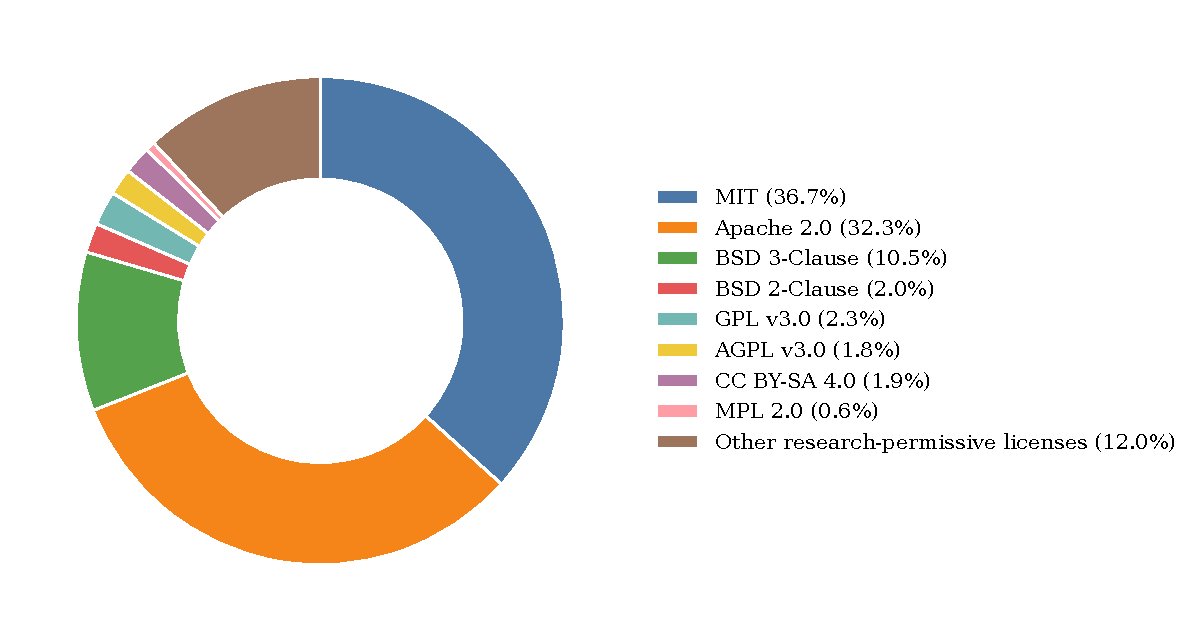
\includegraphics[width=0.85\linewidth]{figs/license_distribution.pdf}
\caption{License distribution of the $968$-repository corpus. Permissive
licenses (MIT, Apache-2.0, BSD) account for over $80\%$ of the corpus.
Small categories (LGPL, ISC, Boost, MIT-0, Unlicense, CC0, CC BY,
CC BY-NC, etc.) are aggregated as ``Other research-permissive licenses,''
all of which permit at least non-commercial research use.}
\label{fig:licenses}
\end{figure}

% =============================================================================
\section{Algorithmic Details}
\label{app:algo}

This appendix collects the full algorithmic details summarized in
Section~\ref{sec:method:selection}.

\subsection{Single-Function FIM Target Selection}
\label{app:algo:single}

Algorithm~\ref{alg:selection} summarizes the per-file pipeline that
produces single-function FIM targets. It composes the program
dependency graph (Section~\ref{sec:method:pdg}), the complexity score
$\hat{H}$ (Section~\ref{sec:method:complexity}), the inferability score
$\hat{I}$ (Section~\ref{sec:method:inferability}), the difficulty
penalty $\rho$ (Appendix~\ref{app:algo:penalty}), and the hard filters
described below.

\begin{algorithm}[h]
\caption{Single-function FIM target selection for one file.}
\label{alg:selection}
\begin{algorithmic}[1]
  \Require Source file $s$; thresholds $\tau_d, \tau_{\mathrm{FIM}}, \tau_{\hat H}$
  \State $T \gets \mathrm{ParseAST}(s)$
  \State $\mathcal{V}, \mathcal{E}_{\mathrm{call}}, \mathcal{E}_{\mathrm{sib}} \gets \mathrm{BuildPDG}(T)$
        \Comment{Section~\ref{sec:method:pdg}}
  \State $\mathcal{C} \gets \emptyset$
  \For{each $v \in \mathcal{V}$}
    \If{$v$ is a dunder method \textbf{or} $\mathrm{LoC}(v) \notin [10, 200]$}
      \State \textbf{continue}
    \EndIf
    \State Compute $\hat{H}(v)$ and $\hat{I}(v)$
          \Comment{Eqs.~\eqref{eq:complexity}, \eqref{eq:inferability}}
    \If{$\hat{H}(v) < \tau_{\hat H}$} \textbf{continue} \EndIf
    \State $\Delta(v) \gets \max(0, \hat{H}(v)-\hat{I}(v)) / (\hat{H}(v)+\epsilon)$
    \State $\mathrm{FIM}(v) \gets \dfrac{\hat{H}(v)\,\hat{I}(v)}{\hat{H}(v)+\hat{I}(v)+\epsilon}\cdot \rho(\Delta(v))$
    \If{$\mathrm{FIM}(v) \ge \tau_{\mathrm{FIM}}$}
      \State $\mathcal{C} \gets \mathcal{C} \cup \{v\}$
    \EndIf
  \EndFor
  \State \Return $\mathcal{C}$ \Comment{ranked by $\mathrm{FIM}$ descending}
\end{algorithmic}
\end{algorithm}

\subsection{Program Dependency Graph: Call Resolution}
\label{app:algo:pdg}

For every \texttt{Call} node inside the body of $u \in \mathcal{V}$, we
attempt to resolve its callee to some $v \in \mathcal{V}$, adding a
directed edge $u \to v$ in $\mathcal{E}_{\mathrm{call}}$. Resolution
handles three Python idioms:
\begin{itemize}\setlength\itemsep{0.1em}
  \item \textbf{Direct module-level invocations}: \texttt{foo(...)} is
        resolved by qualified-name lookup in the same module.
  \item \textbf{Class instantiation}: \texttt{ClassName(...)} is
        resolved to \texttt{ClassName.\_\_init\_\_}.
  \item \textbf{Method calls}: \texttt{self.m(...)} or \texttt{cls.m(...)}
        inside class bodies is resolved within the enclosing class scope.
\end{itemize}
When a call cannot be resolved exactly we fall back to short-name
matching against the qualified-name index, which recovers most
cross-module references while admitting a controlled false-positive rate.
Sibling edges $\mathcal{E}_{\mathrm{sib}}$ are constructed by
enumerating all pairs of methods belonging to the same class.

\subsection{Complexity Score: Caps and Weights}
\label{app:algo:hyperparams}

The complexity score $\hat{H}(v)$ defined in Eq.~\eqref{eq:complexity}
uses caps $(c_{\ell}, c_{c}, c_{d}) = (50, 10, 5)$ and weights
$(w_{\ell}, w_{c}, w_{d}) = (0.4, 0.4, 0.2)$. The cap $c_{\ell}=50$
on lines of code matches the median target length in our corpus; the
cap $c_c=10$ on McCabe complexity is roughly twice the median over our
filtered functions; the cap $c_d=5$ on nesting depth covers the tail of
practical Python code. The cap value of $2$ in $\phi(x,c)=\min(x/c,2)$
allows genuinely complex functions to score above the median without
letting outliers dominate.

\subsection{Inferability Score: Component Formulas}
\label{app:algo:inferability}

The five components of $\hat{I}(v)$ (Eq.~\ref{eq:inferability}) are
defined below. Default mixing weights are
$(\alpha,\beta,\gamma,\delta,\varepsilon) = (0.30, 0.25, 0.20, 0.10, 0.15)$.

\textbf{Caller signal $C_{\mathrm{caller}}$.}
For each caller $u$ of $v$, we score the specificity of its call sites
by inspecting the syntactic form of each argument: literal constants are
maximally informative, named variables less so, keyword arguments
contribute proportionally, and a base score is awarded for the call
site itself. The sum is normalized by an expected-callers constant.

\textbf{Callee signal $C_{\mathrm{callee}}$.}
The number of intra-file functions that $v$ itself calls, normalized by
a small expected-fan-out constant. A function that orchestrates known
helpers is more recoverable than one calling only opaque externals.

\textbf{Signature signal $C_{\mathrm{sig}}$.}
A monotone aggregate of return-type annotation, parameter-type
annotations, the descriptiveness of the function name (decomposed into
snake-case parts), and the count of non-\texttt{self} parameters.

\textbf{Documentation signal $C_{\mathrm{doc}}$.}
Indicator of docstring presence. We do not score docstring
informativeness, both for robustness and because
Section~\ref{sec:method:cot} generates a richer textual rationale.

\textbf{Class signal $C_{\mathrm{class}}$.}
For methods, the number of in-class siblings (normalized) plus a small
bonus when an \texttt{\_\_init\_\_} is present in the same class.

\subsection{Difficulty $\Delta$, Penalty $\rho$, and Hard Filters}
\label{app:algo:penalty}

The penalty $\rho(\Delta(v))$ in Eq.~\eqref{eq:fim_single} is built from
the residual difficulty $\Delta(v)$, defined as the share of complexity
that is not explained by context:
\begin{equation}
  \Delta(v) \;=\; \frac{\max\!\left(0,\,\hat{H}(v) - \hat{I}(v)\right)}{\hat{H}(v) + \epsilon}
  \;\in\; [0, 1).
  \label{eq:delta}
\end{equation}
The penalty $\rho$ is one-sided: targets with $\Delta(v) \le \tau_d$ are
left intact, while targets above the threshold are damped by a Gaussian
factor:
\begin{equation}
  \rho(\Delta) \;=\;
  \begin{cases}
    1, & \Delta \le \tau_d, \\[2pt]
    \exp\!\left(-\dfrac{(\Delta - \tau_d)^2}{2\sigma^2}\right), & \Delta > \tau_d.
  \end{cases}
  \label{eq:penalty}
\end{equation}
We use $\tau_d = 0.5$ and $\sigma = 0.2$. The asymmetry reflects an
asymmetry in the underlying objective: trivially easy targets are
already eliminated by the hard filters below, so we do not need to
additionally reward high inferability; conversely, targets that remain
hard even with full context become unlearnable noise and must be
down-weighted.

\textbf{Hard filters.}
Independent of the smooth score, we discard \emph{(i)} functions with
$\mathrm{LoC}(v) \notin [10, 200]$ to control training-instance length;
\emph{(ii)} dunder methods (\texttt{\_\_init\_\_},
\texttt{\_\_repr\_\_}, etc.), which serve as scaffolding rather than
reasoning targets; \emph{(iii)} functions with $\hat{H}(v) < 0.15$ to
remove trivial cases; and \emph{(iv)} functions with
$\mathrm{FIM}(v) < 0.08$. A file with no surviving target contributes
nothing to the corpus.

\subsection{Worked Example: Scoring \texttt{Calculator.total}}
\label{app:algo:worked_example}

To make the numbers in Figure~\ref{fig:pdg_score}(b) reproducible, this
subsection walks through every quantity that goes into $\hat{H}$,
$\hat{I}$, and the final FIM score for the running example. The target
function is:

\begin{center}\small
\begin{minipage}{0.78\linewidth}
\begin{verbatim}
def total(self) -> int:
    """Sum positive integer entries."""
    s, n = 0, 0
    for v in self.history:
        if is_int(v):
            if v > 0:
                s = add(s, v)
                n += 1
    if n == 0: return 0
    return s
\end{verbatim}
\end{minipage}
\end{center}

\textbf{Lines of code (LoC = 10).}
Following Python's \texttt{ast} convention,
$\mathrm{LoC}(v)=\texttt{end\_lineno}-(\texttt{lineno}-1)$, the number
of source lines from the \texttt{def} keyword through the last
statement, both inclusive. Counting the ten lines above (including the
docstring) gives $\mathrm{LoC}=10$.

\textbf{Cyclomatic complexity (CC = 5).}
The McCabe counter starts at $1$ and adds $1$ per branching node:
\texttt{If}/\texttt{IfExp}, \texttt{For}/\texttt{While},
\texttt{ExceptHandler}, $(\text{values}{-}1)$ per \texttt{BoolOp}, and
one per generator inside a comprehension. For
\texttt{Calculator.total}: base ($+1$), the \texttt{for} loop ($+1$),
\texttt{if is\_int} ($+1$), \texttt{if v>0} ($+1$), \texttt{if n==0}
($+1$), totalling $\mathrm{CC}=5$. Tuple unpacking and \texttt{n+=1}
are not branches.

\textbf{Maximum nesting depth (D = 3).}
Depth increments only on structural containers (\texttt{If},
\texttt{For}, \texttt{While}, \texttt{AsyncFor}, \texttt{With},
\texttt{AsyncWith}, \texttt{Try}). The deepest path in
\texttt{total} is \texttt{for}~$\to$~\texttt{if is\_int}~$\to$~%
\texttt{if v>0}, giving $\mathrm{D}=3$.

\textbf{Complexity score $\hat{H}=0.40$.}
Plugging into Eq.~\ref{eq:complexity} with the default
$(w_{\ell},w_{c},w_{d})=(0.4,0.4,0.2)$ and
$(c_{\ell},c_{c},c_{d})=(50,10,5)$:
\begin{align*}
w_{\ell}\,\phi(10,50) &= 0.4\!\cdot\!0.20 = 0.08, \qquad
w_{c}\,\phi(5,10)     = 0.4\!\cdot\!0.50 = 0.20, \\
w_{d}\,\phi(3,5)      &= 0.2\!\cdot\!0.60 = 0.12, \quad
\hat{H}(\texttt{total}) = 0.08+0.20+0.12 = 0.40.
\end{align*}

\textbf{Inferability score $\hat{I}=0.48$.}
\emph{(i)~Caller specificity.} The only in-file caller is
\texttt{Calculator.mean}, which invokes \texttt{self.total()} with no
arguments. The specificity routine assigns $0.50$ for the call site,
$0$ for arguments and keywords, and a $+0.10$ found bonus, yielding
$\mathrm{sp}=0.60$. Aggregating over callers and normalizing by $3$,
$C_{\mathrm{caller}}=\min(0.60/3,1.0)=0.20$ and
$\alpha\,C_{\mathrm{caller}}=0.06$.
\emph{(ii)~Callee count.} \texttt{total} calls \texttt{is\_int} and
\texttt{add} in-file (\texttt{self.history.append(v)} does not count
because \texttt{append} is not in $\mathcal{V}$), so
$C_{\mathrm{callee}}=\min(2/4,1.0)=0.50$ and
$\beta\,C_{\mathrm{callee}}=0.13$.
\emph{(iii)~Signature.} Sub-bonuses $+0.30$ for \texttt{-> int},
$+0.20$ for the descriptive name \texttt{total}, $0$ for parameter type
annotations, $0$ for non-\texttt{self} parameters: $C_{\mathrm{sig}}=0.50$
and $\gamma\,C_{\mathrm{sig}}=0.10$.
\emph{(iv)~Documentation.} A docstring is present, so
$C_{\mathrm{doc}}=0.5$ and $\delta\,C_{\mathrm{doc}}=0.05$.
\emph{(v)~Class context.} \texttt{total} sits among three siblings;
the base score is $\min(3/5,1.0)=0.60$, plus a $+0.30$ bonus for the
distinct \texttt{\_\_init\_\_} of \texttt{Calculator}, giving
$C_{\mathrm{class}}=0.90$ and $\varepsilon\,C_{\mathrm{class}}=0.14$.
Summing: $\hat{I}(\texttt{total})=0.06+0.13+0.10+0.05+0.14=0.48$.

\textbf{Final FIM score and selection.}
$\Delta(\texttt{total})=\max(0,-0.08)/0.40=0$, so
$\rho(\Delta)=1$ and
$\mathrm{FIM}(\texttt{total})=(0.40\!\cdot\!0.48)/(0.40\!+\!0.48)\approx 0.22 \geq \tau\!=\!0.20$,
selecting it as a mask target. The four short helpers are removed before
scoring by the LoC hard filter; \texttt{Calculator.\_\_init\_\_} is
removed by the dunder filter.

\subsection{Multi-Function Group Score}
\label{app:algo:groups}

\textbf{Group score.}
For a group $G = \{v_1, \dots, v_k\}$ enumerated from one of eight
topology patterns,
\begin{equation}
  \mathrm{FIM}(G) \;=\;
  \mathrm{Coup}(G)
  \cdot
  \frac{\hat{H}(G)\,\hat{I}(G)}{\hat{H}(G) + \hat{I}(G) + \epsilon}
  \cdot
  \rho\!\left(\Delta(G)\right),
  \label{eq:fim_group}
\end{equation}
where $\hat{H}(G)=\tfrac{1}{k}\sum_v \hat{H}(v)$ averages individual
complexities, $\Delta(G)$ is defined analogously to the single-function
case, and the coupling term $\mathrm{Coup}(G)\in[0,1]$ is a normalized
count of intra-group edges plus a shared-state ratio:
\begin{equation}
  \mathrm{Coup}(G)
  \;=\; w_{\mathrm{c}}\,\frac{|E^{\text{call}}_G|}{k(k\!-\!1)}
   + w_{\mathrm{s}}\,\frac{|E^{\text{sib}}_G|}{\binom{k}{2}}
   + w_{\mathrm{st}}\,\overline{\mathrm{Jacc}}_G,
  \label{eq:coupling}
\end{equation}
with $\overline{\mathrm{Jacc}}_G$ the mean Jaccard similarity over pairs
in $G$ between sets of accessed instance attributes (\texttt{self.x}).
We use $(w_{\mathrm{c}}, w_{\mathrm{s}}, w_{\mathrm{st}}) = (0.50,
0.20, 0.30)$. The coupling term enters multiplicatively because, unlike
the single-function case, the value of a multi-function target derives
specifically from cross-function dependencies; a weakly coupled group
is indistinguishable from $k$ independent samples.

\textbf{Group inferability.}
$\hat{I}(G)$ is recomputed under the assumption that \emph{all} members
of $G$ are masked simultaneously: caller, callee, and sibling
contributions from inside $G$ are excluded, and docstrings of group
members contribute zero (they are part of the masked body). Signature
information is retained because we do not mask function signatures.
This re-computation prevents groups from receiving spurious credit for
intra-group references that disappear under joint masking.

\textbf{Topology taxonomy.}
A candidate group must form a connected subgraph in
$\mathcal{E}_{\mathrm{call}} \cup \mathcal{E}_{\mathrm{sib}}$. We
enumerate eight patterns:
\begin{itemize}\setlength\itemsep{0.1em}
  \item \emph{$k=2$}: \emph{caller-callee} (direct $A\!\to\!B$ edge);
  \emph{co-callee} (two callees of a common caller); \emph{sibling-coupled}
  (same-class methods sharing $\geq 1$ instance attribute);
  \emph{mutual-call} ($A\!\rightleftharpoons\!B$).
  \item \emph{$k=3$}: \emph{call-chain} ($A\!\to\!B\!\to\!C$); \emph{hub}
  ($A\!\to\!B,\ A\!\to\!C$); \emph{fan-in} ($B\!\to\!A,\ C\!\to\!A$);
  \emph{class-triad} (three pairwise state-sharing methods of the same
  class).
\end{itemize}

\textbf{Group selection.}
We score every candidate group emitted by the topology enumerator and
discard those with insufficient coupling, complexity, or score
(defaults: $\mathrm{Coup}(G) \ge 0.20$; $\hat{H}(G) \ge 0.18$;
$\mathrm{FIM}(G) \ge 0.10$). Groups exceeding LoC ratios of $0.30$
($k=2$) or $0.40$ ($k=3$) of the file are rejected. Remaining
candidates are sorted by $\mathrm{FIM}(G)$ and selected greedily under
non-overlap: a function may belong to at most one selected group per
file. Per-file caps ($5$ pairs, $3$ triples) prevent any single file
from dominating the corpus.

\begin{algorithm}[h]
\caption{Multi-function group FIM target selection for one file.}
\label{alg:selection_multi}
\begin{algorithmic}[1]
  \Require Source file $s$; per-function scores $\hat{H}(v),\hat{I}(v)$;
           thresholds $\tau^G_{\mathrm{coup}}, \tau^G_{\hat H}, \tau^G_{\mathrm{FIM}}$;
           per-file caps $(N_2, N_3)=(5, 3)$
  \State $\mathcal{V}, \mathcal{E}_{\mathrm{call}}, \mathcal{E}_{\mathrm{sib}} \gets \mathrm{BuildPDG}(\mathrm{ParseAST}(s))$
  \State $\mathcal{G} \gets \emptyset$
  \For{each topology pattern $P \in \{\text{caller-callee, co-callee, sibling-coupled, mutual-call,}$
       $\quad\text{call-chain, hub, fan-in, class-triad}\}$}
    \State Enumerate all connected subgraphs $G \subseteq \mathcal{V}$ matching $P$
           in $\mathcal{E}_{\mathrm{call}}\cup\mathcal{E}_{\mathrm{sib}}$
    \For{each candidate $G$}
      \If{$\mathrm{LoC\_ratio}(G,s)>\theta_k$ \textbf{or}
          $\mathrm{Coup}(G)<\tau^G_{\mathrm{coup}}$ \textbf{or}
          $\hat{H}(G)<\tau^G_{\hat H}$}
        \State \textbf{continue}
      \EndIf
      \State Recompute $\hat{I}(G)$ under joint masking
            \Comment{exclude intra-group references}
      \State $\Delta(G) \gets \max(0, \hat{H}(G)-\hat{I}(G))/(\hat{H}(G)+\epsilon)$
      \State $\mathrm{FIM}(G) \gets \mathrm{Coup}(G)\cdot
              \dfrac{\hat{H}(G)\,\hat{I}(G)}{\hat{H}(G)+\hat{I}(G)+\epsilon}\cdot \rho(\Delta(G))$
      \If{$\mathrm{FIM}(G) \ge \tau^G_{\mathrm{FIM}}$}
        \State $\mathcal{G} \gets \mathcal{G} \cup \{(G,P,\mathrm{FIM}(G))\}$
      \EndIf
    \EndFor
  \EndFor
  \State Sort $\mathcal{G}$ by $\mathrm{FIM}(G)$ descending
  \State $\mathcal{S} \gets \emptyset$
  \For{each $(G,P,\mathrm{FIM}(G)) \in \mathcal{G}$}
    \If{any $v \in G$ already covered by $\mathcal{S}$
        \textbf{or} per-pattern cap $(N_2$ for $k\!=\!2$, $N_3$ for $k\!=\!3)$ exceeded}
      \State \textbf{continue}
    \EndIf
    \State $\mathcal{S} \gets \mathcal{S} \cup \{G\}$
  \EndFor
  \State \Return $\mathcal{S}$
\end{algorithmic}
\end{algorithm}

\subsection{Worked Example: A \texttt{caller-callee} Pair}
\label{app:algo:groups_example}

To illustrate the group score, consider a small file with two
top-level functions:

\begin{center}\small
\begin{minipage}{0.82\linewidth}
\begin{verbatim}
def normalize(text: str) -> str:
    """Lowercase and strip punctuation."""
    out = []
    for ch in text:
        if ch.isalnum() or ch.isspace():
            out.append(ch.lower())
    return "".join(out)

def word_freq(doc: str) -> dict[str, int]:
    """Count tokens of `doc` after normalization."""
    cleaned = normalize(doc)
    counts = {}
    for tok in cleaned.split():
        counts[tok] = counts.get(tok, 0) + 1
    return counts
\end{verbatim}
\end{minipage}
\end{center}

\textbf{Topology and pre-checks.} The pair
$G\!=\!\{\texttt{normalize}, \texttt{word\_freq}\}$ matches the
\emph{caller-callee} pattern with one call edge
$\texttt{word\_freq}\!\to\!\texttt{normalize}$. They are top-level
(no class), so the sibling component of $\mathrm{Coup}$ is zero and
the shared-state component is zero (no \texttt{self.\_}~accesses). The
combined LoC is roughly $14$ lines, well under the $\theta_2\!=\!0.30$
file-ratio cap.

\textbf{Coupling.} With one call edge in a pair,
$|E^{\text{call}}_G|/(k(k\!-\!1))=1/2$. Plugging into
Eq.~\ref{eq:coupling} with $(w_c,w_s,w_{st})=(0.50,0.20,0.30)$:
$\mathrm{Coup}(G)=0.50\cdot 0.5+0+0=0.25$, comfortably above the
$\tau^G_{\mathrm{coup}}=0.20$ floor.

\textbf{Group $\hat{H}$.} Per-function complexities (computed as in
Section~\ref{sec:method:complexity}) come out to roughly
$\hat{H}(\texttt{normalize})\!\approx\!0.36$ (LoC=$7$, CC=$3$, D=$2$)
and $\hat{H}(\texttt{word\_freq})\!\approx\!0.30$ (LoC=$7$, CC=$2$,
D=$2$), giving $\hat{H}(G)\!\approx\!0.33$.

\textbf{Group $\hat{I}$ under joint masking.} Both functions are
masked, so the call edge between them no longer contributes to
$C_{\mathrm{caller}}$ or $C_{\mathrm{callee}}$. Signature information
is retained: both have descriptive names and full type annotations
(strong $C_{\mathrm{sig}}$); both have docstrings (small but nonzero
$C_{\mathrm{doc}}$). With no surviving caller/callee/class signal, the
group inferability collapses to $\hat{I}(G)\!\approx\!0.18$, dominated
by the signature term.

\textbf{Final group FIM.} The harmonic-mean-like product
$\hat{H}\hat{I}/(\hat{H}+\hat{I})\!\approx\!(0.33\!\cdot\!0.18)/0.51\!\approx\!0.116$,
$\Delta(G)\!=\!(0.33-0.18)/0.33\!\approx\!0.45<\tau_d=0.5$ so
$\rho=1$, and $\mathrm{Coup}(G)=0.25$:
$\mathrm{FIM}(G)\approx 0.25\!\times\!0.116\!\approx\!0.029$. This
example sits below the $\tau^G_{\mathrm{FIM}}\!=\!0.10$ floor and would
therefore \emph{not} be selected---the toy module is too small for the
joint-masking inferability to remain large enough. Real corpus pairs
that pass the threshold typically come from class-method pairs with
non-trivial sibling and shared-state coupling, where $\hat{I}(G)$
retains substantial $C_{\mathrm{class}}$ contribution even under joint
masking. The walkthrough nonetheless shows the mechanism: joint masking
strictly reduces $\hat{I}$ relative to the single-function average,
and the coupling factor must compensate.

\subsection{Chain-of-Thought Prompt Template}
\label{app:algo:cot}

The chain-of-thought rationale embedded inside each FIM middle span
(Section~\ref{sec:method:cot}) is generated by Gemini-3-Flash using
the following prompt skeleton:

\begin{quote}\small
\textit{[System]} You are an expert software engineer.

\noindent\textit{[User]} Below is a Python source file with one function
body redacted (shown as \texttt{<MASKED>}).

\noindent\texttt{<file with target body redacted>}

\noindent The redacted function has the following signature and (if
present) docstring:

\noindent\texttt{<signature + docstring>}

\noindent The original function body was:

\noindent\texttt{<original body>}

\noindent Write a concise step-by-step rationale (in natural language)
that explains how the body's behavior could be \textbf{recovered} from
the surrounding file---for example, by referencing call sites, helper
functions, and class-level state---without simply restating the code.
\end{quote}

Rationales are constrained to at most $300$ tokens and are filtered by
length and basic format checks before training. We use greedy decoding;
retry logic and quality filters will be released with the corpus.

\subsection{Negative-Observation Patterns}
\label{app:algo:neg_patterns}

The recovery-rate analysis (Section~\ref{sec:analysis:recovery}) flags
a tool output as a \emph{negative observation} when it matches any of
the following patterns: Python stack-trace prefixes
(\texttt{Traceback (most recent call last):}); error class names
(\texttt{SyntaxError}, \texttt{IndentationError}, \texttt{NameError},
\texttt{ImportError}, \texttt{AttributeError}, \texttt{TypeError},
\texttt{ValueError}); shell error markers
(\texttt{command not found}, \texttt{permission denied}, \texttt{No such file or directory});
and harness-specific failure strings
(\texttt{No replacement was performed}, \texttt{Patch did not apply},
\texttt{tests failed}). Patterns are matched case-insensitively.

% =============================================================================
\section{Training Hyperparameters}
\label{app:hp}

We use \textsc{LlamaFactory} for FIM mid-training, R2E-Gym
post-training, and SWE-Lego post-training, and \textsc{torchtune} for
SWE-Smith post-training. All runs use AdamW with bf16 mixed precision
and a cosine learning-rate schedule. For R2E-Gym and SWE-Smith we follow
the official release scripts; for SWE-Lego we use $2$ epochs instead of
the official $4$ to prevent overfitting (all other hyperparameters
unchanged). Tables~\ref{tab:hp-midtrain} and~\ref{tab:hp-posttrain} list
the exact settings; effective (global) batch sizes assume $8$ GPUs.

\begin{table}[h]
\centering
\footnotesize
\caption{FIM mid-training hyperparameters, applied uniformly to all
three base models (Qwen2.5-Coder-7B-Instruct,
Qwen2.5-Coder-14B-Instruct, and Qwen3-8B).}
\label{tab:hp-midtrain}
\setlength{\tabcolsep}{8pt}
\begin{tabular}{ll}
\toprule
\textbf{Hyperparameter} & \textbf{Value} \\
\midrule
Optimizer             & AdamW \\
Learning rate         & $1.0\!\times\!10^{-5}$ \\
LR schedule           & Cosine \\
Warmup ratio          & $0.1$ \\
Weight decay          & $0.05$ \\
Epochs                & $1$ \\
Per-device batch size & $1$ \\
Gradient accumulation & $16$ \\
Effective batch size  & $128$ \\
Sequence length       & $32{,}768$ \\
Precision             & bf16 \\
\bottomrule
\end{tabular}
\end{table}

\begin{table}[h]
\centering
\footnotesize
\caption{Agentic post-training hyperparameters for the three pipelines.
R2E-Gym and SWE-Smith follow their official released scripts; SWE-Lego
follows the official recipe except for the epoch count.}
\label{tab:hp-posttrain}
\setlength{\tabcolsep}{6pt}
\begin{tabular}{lccc}
\toprule
\textbf{Hyperparameter} & \textbf{R2E-Gym} & \textbf{SWE-Smith} & \textbf{SWE-Lego} \\
\midrule
Base model            & Qwen2.5-Coder-7B-Inst.
                      & Qwen2.5-Coder-7B-Inst.
                      & Qwen3-8B (FIM-midtrained) \\
Optimizer             & AdamW & AdamW (fused) & AdamW \\
Learning rate         & $1.0\!\times\!10^{-5}$
                      & $1.0\!\times\!10^{-4}$
                      & $1.0\!\times\!10^{-4}$ \\
LR schedule           & Cosine & Cosine & Cosine \\
Warmup                & ratio $0.05$ & $5$ steps & ratio $0.1$ \\
Weight decay          & $0.0$ & $0.01$ & $0.01$ \\
Epochs                & $2$ & $3$ & $2$\textsuperscript{$\dagger$} \\
Per-device batch size & $1$ & $1$ & $1$ \\
Gradient accumulation & $1$ & $4$ & $8$ \\
Effective batch size  & $8$ & $32$ & $64$ \\
Sequence length       & $32{,}768$ & $32{,}768$ & $40{,}960$ \\
Precision             & bf16 & bf16 & bf16 \\
\bottomrule
\end{tabular}
\\[0.3em]
{\raggedright \footnotesize \textsuperscript{$\dagger$}Deviates from the
official SWE-Lego recipe ($4$ epochs); reduced to $2$ to prevent
overfitting on the FIM-midtrained Qwen3-8B base.\par}
\end{table}

\subsection{Compute Resources}
\label{app:hp:compute}
All experiments are run on a single node of $8$ NVIDIA H100 80\,GB GPUs.
Reproducing the full set of results in this paper---FIM mid-training
of three base models (Qwen2.5-Coder-7B/14B-Instruct and Qwen3-8B), the
three agentic post-training pipelines (R2E-Gym, SWE-Smith, SWE-Lego)
and their corresponding mid-trained variants, the data/CoT/granularity
ablations of Section~\ref{sec:exp:abl}, and the multi-seed evaluation
sweeps---takes roughly $30$ days of wall-clock time on the $8$-GPU node,
i.e.\ $\approx\!5{,}760$ GPU-hours in total. Preliminary and discarded
runs not reported in this paper account for an additional ${\sim}30\%$
of compute.

% =============================================================================
\section{Extended Behavioral Analysis (SWE-Bench-Verified)}
\label{app:behavior_extra}

This appendix collects the trajectory-level material that supplements
the headline analysis in Section~\ref{sec:analysis}. Unless stated
otherwise, statistics are run-means over three independent evaluation
runs of each checkpoint on SWE-Bench-Verified ($500$ instances per run).

\subsection{Pass Rate by Gold-Patch Shape}
\label{app:behavior_extra:patchshape}

Figure~\ref{fig:patchshape} reports the pass-rate stratification used
in Section~\ref{sec:analysis:multifn}: the largest gain
($+9.1$~pp) is on multi-function single-file tasks
($n{=}88$), more than $4{\times}$ the $+2.1$~pp gain on single-function
tasks ($n{=}341$); multi-file tasks ($n{=}71$) remain hard for both
checkpoints ($\sim\!11.3\%$ each).

\begin{figure}[h]
\centering
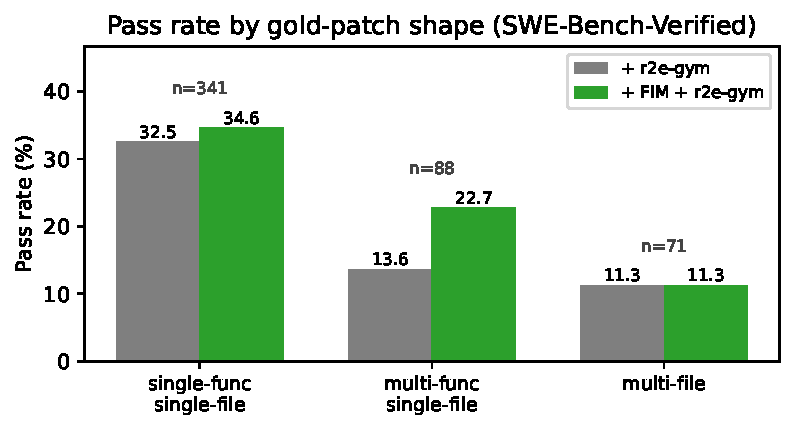
\includegraphics[width=0.62\linewidth]{figs/passrate_by_patchshape_verified.pdf}
\caption{Pass rate on SWE-Bench-Verified ($14$B + R2E-Gym) stratified
by gold-patch shape, run-means over three evaluation runs per
checkpoint.}
\label{fig:patchshape}
\end{figure}

\subsection{Full Trajectory Metrics}
\label{app:behavior_extra:metrics}

Table~\ref{tab:behavior_full} reports the full trajectory metrics
summarized in Table~\ref{tab:behavior_main}, including unsolved-task
breakdowns and output/context summaries.

\begin{table}[h]
\centering
\caption{Trajectory-level behavioral metrics on SWE-Bench-Verified
(14B, R2E-Gym), run-means over three evaluation runs of each
checkpoint. Steps, edits, and errors-encountered are means per task.
``Empty patch'' is the fraction of \emph{failed} trajectories whose
final \texttt{output\_patch} is empty; ``Loc.\ correct'' is the
fraction of all trajectories that locate at least one file overlapping
the gold patch; ``Ctx @ success'' is the mean prompt context length on
solved trajectories.}
\label{tab:behavior_full}
\small
\setlength{\tabcolsep}{4pt}
\begin{tabular}{l c c c c c c c}
\toprule
& \multicolumn{2}{c}{Steps / task}
& \multicolumn{2}{c}{Edits / task}
& \multicolumn{2}{c}{Errors enc.}
& Recovery \\
\cmidrule(lr){2-3}\cmidrule(lr){4-5}\cmidrule(lr){6-7}
Setting & solved & unsolved & solved & unsolved & solved & unsolved & rate (\%) \\
\midrule
+ R2E-Gym
  & 15.1 & 22.4 & 3.3 & 5.4 & 3.5 & 5.8 & 24.8 \\
\textbf{+ FIM-Midtrain + R2E-Gym}
  & \textbf{23.6} & \textbf{32.7} & \textbf{7.4} & \textbf{10.9}
  & \textbf{6.2} & \textbf{8.1} & \textbf{28.8} \\
\midrule
\multicolumn{8}{l}{\textit{Output and context summaries}} \\
\midrule
& \multicolumn{2}{c}{Empty patch (\% failed)}
& \multicolumn{2}{c}{Loc.\ correct (\% all)}
& \multicolumn{2}{c}{Ctx @ success (tok)}
& Pass (\%) \\
\cmidrule(lr){2-3}\cmidrule(lr){4-5}\cmidrule(lr){6-7}
+ R2E-Gym
  & \multicolumn{2}{c}{$3.0$} & \multicolumn{2}{c}{$70.6$}
  & \multicolumn{2}{c}{$11{,}826$} & 26.2 \\
\textbf{+ FIM-Midtrain + R2E-Gym}
  & \multicolumn{2}{c}{$\mathbf{0.3}$} & \multicolumn{2}{c}{$\mathbf{73.4}$}
  & \multicolumn{2}{c}{$\mathbf{16{,}397}$} & \textbf{29.2} \\
\bottomrule
\end{tabular}
\end{table}

\subsection{Iterate-and-Verify: Action-Type Distribution}
\label{app:behavior_extra:actions}

Mid-training shifts the action-type distribution toward an
iterate-and-verify policy. The share of \texttt{search} actions falls
from $15.3\%$ to $11.0\%$, while the share of \texttt{execute\_bash}
actions rises from $19.5\%$ to $24.6\%$: the agent spends a smaller
fraction of its budget on passive repository lookup and a larger
fraction on actively running scripts and tests, then refining its
edit. The cost is more steps---ours hits the step cap on $\sim\!45\%$
of trajectories vs.\ $7\%$ for the baseline---but this cost is paid on
the unsolved tail; on the solved set the additional steps translate
into more correct patches.

\subsection{Failure-Mode Breakdown}
\label{app:behavior_extra:failure}

We label every failed trajectory using a deterministic patch-quality
cascade: \emph{no-patch} (output diff is empty); \emph{localization
error} (non-empty patch but zero file overlap with the gold patch);
\emph{patch error} (file overlap with gold patch but tests fail).
Figure~\ref{fig:failure_app} reports the outcome distribution: across
the three runs, mid-training cuts no-patch failures by an order of
magnitude ($\sim\!11\!\to\!\sim\!1$ trajectories per run), trims
localization errors slightly ($\sim\!131\!\to\!\sim\!126$), and leaves
the patch-error count essentially flat ($\sim\!227\!\to\!\sim\!227$).
The $+15$-task gain in solved count is therefore primarily driven by
the no-patch mode collapse.

\begin{figure}[h]
\centering
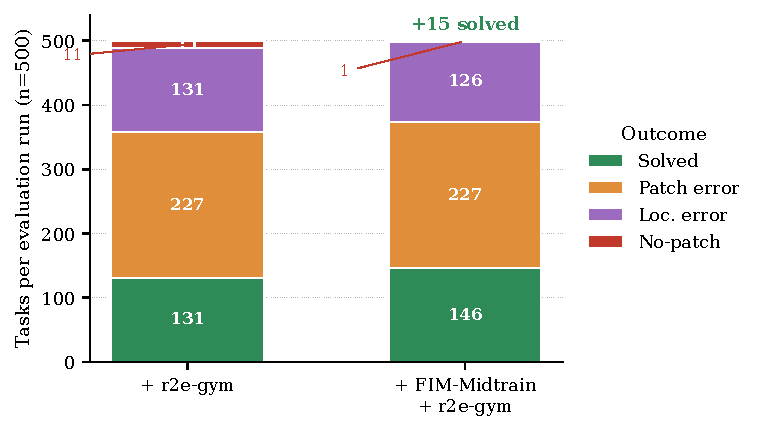
\includegraphics[width=0.55\linewidth]{figs/failure_modes.pdf}
\caption{Outcome distribution per evaluation run on SWE-Bench-Verified
(14B, R2E-Gym), averaged over three runs.}
\label{fig:failure_app}
\end{figure}

\subsection{No-Patch Mode: Mechanism}
\label{app:behavior_extra:nopatch}

The baseline no-patch failures recovered by mid-training are
distributed across all task buckets and are not concentrated in any
single repository. In every recovered case the baseline emitted
\texttt{<finish>} without applying any \texttt{str\_replace}, while
ours applied at least one edit. We interpret this as a direct
consequence of the FIM training signal: under FIM the model is always
conditioned to produce a non-empty token span between the prefix and
suffix, and this disposition survives the post-training pipeline.

\subsection{Multi-File Tasks Are Not Differentially Helped}
\label{app:behavior_extra:multifile}

On the $71$ Verified tasks whose gold patch spans $\geq 2$ files, both
checkpoints solve $\sim\!11.3\%$ on average and per-instance
head-to-head on this bucket is balanced. We attribute this to a
granularity mismatch: our function-aware FIM mid-training operates at
the function level within files, so cross-file coordination is not
directly trained for. Extending the selection algorithm to cross-file
function pairs is a natural follow-up.

\subsection{A Concrete Contrast}
\label{app:behavior_extra:contrast}

The shift in termination behavior is clearest on cases where the
baseline quits prematurely. On \texttt{scikit-learn-26323}, for
instance, the baseline trajectory runs for a single step in every run,
immediately emits \texttt{<finish>} with an empty edit and the wrong
target file, and is scored as a failure; on the same task our agent
runs $\sim\!41$ steps, applies on the order of $20$
\texttt{str\_replace} operations, observes multiple negative tool
returns, and recovers to a passing patch. Pooling across the three
runs, on the order of $\sim\!16$ of the $\sim\!55$ tasks that ours
uniquely solves on Verified have this signature: the baseline emits
\texttt{<finish>} with zero file overlap with the gold patch (often
before any negative observation has even arrived), while ours iterates
past intermediate signals and converges on a correct edit.
Mid-training does not enable a categorically new capability on these
instances; it changes the agent's stopping policy.

% =============================================================================
\section{Behavioral Analysis on SWE-Bench-Lite}
\label{app:behavior_lite}

This appendix replicates the Verified analysis on the SWE-Bench-Lite
test split ($300$ instances). The same trajectory-parsing pipeline and
failure-mode taxonomy are used; statistics are run-means over three
independent evaluation runs of each checkpoint.

The qualitative trends from Verified hold on Lite: mid-training raises
the recovery rate from $18.8\%$ to $22.1\%$, eliminates the no-patch
failure mode entirely (baseline averages $\sim\!8$ no-patch failures
per run, ours averages $0$), and increases edit iteration on solved
trajectories from $4.4$ to $7.8$ \texttt{str\_replace} operations per
task. The \emph{multi-function} concentration of gain documented on
Verified is not visible on Lite because Lite contains no multi-file
tasks and only $54$ multi-function single-file tasks; the bulk of Lite
is single-function single-file tasks, on which the gain is
$+4.9$~pp ($19.5\%\!\to\!24.4\%$).

\begin{table}[h]
\centering
\caption{Trajectory-level behavioral metrics on SWE-Bench-Lite (14B,
R2E-Gym), run-means over three evaluation runs of each checkpoint.
Definitions match Table~\ref{tab:behavior_full}.}
\label{tab:behavior_lite}
\small
\setlength{\tabcolsep}{4pt}
\begin{tabular}{l c c c c c c c}
\toprule
& \multicolumn{2}{c}{Steps / task}
& \multicolumn{2}{c}{Edits / task}
& \multicolumn{2}{c}{Errors enc.}
& Recovery \\
\cmidrule(lr){2-3}\cmidrule(lr){4-5}\cmidrule(lr){6-7}
Setting & solved & unsolved & solved & unsolved & solved & unsolved & rate (\%) \\
\midrule
+ R2E-Gym
  & 17.5 & 21.3 & 4.4 & 5.2 & 4.8 & 5.4 & 18.8 \\
\textbf{+ FIM-Midtrain + R2E-Gym}
  & \textbf{24.6} & \textbf{31.7} & \textbf{7.8} & \textbf{11.1}
  & \textbf{5.7} & \textbf{7.5} & \textbf{22.1} \\
\midrule
\multicolumn{8}{l}{\textit{Output and context summaries}} \\
\midrule
& \multicolumn{2}{c}{Empty patch (\% failed)}
& \multicolumn{2}{c}{Loc.\ correct (\% all)}
& \multicolumn{2}{c}{Ctx @ success (tok)}
& Pass (\%) \\
\cmidrule(lr){2-3}\cmidrule(lr){4-5}\cmidrule(lr){6-7}
+ R2E-Gym
  & \multicolumn{2}{c}{$3.3$} & \multicolumn{2}{c}{$65.0$}
  & \multicolumn{2}{c}{$13{,}958$} & 18.0 \\
\textbf{+ FIM-Midtrain + R2E-Gym}
  & \multicolumn{2}{c}{$\mathbf{0.0}$} & \multicolumn{2}{c}{$\mathbf{71.0}$}
  & \multicolumn{2}{c}{$\mathbf{18{,}104}$} & \textbf{22.0} \\
\bottomrule
\end{tabular}
\end{table}

Failure-mode counts on Lite move in the same direction as on Verified:
the no-patch mode is eliminated ($\sim\!8\!\to\!0$ trajectories per
run), localization errors fall by about $11$, and patch errors rise by
about $7$, reflecting the same iterate-and-verify shift.

\begin{figure}[h]
\centering
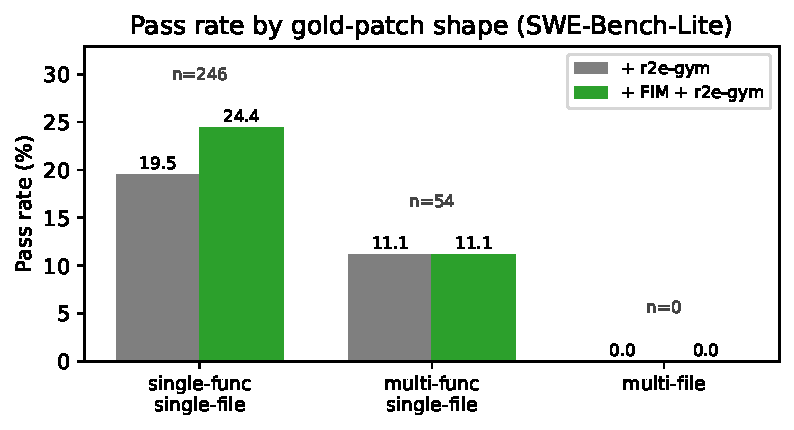
\includegraphics[width=0.62\linewidth]{figs/passrate_by_patchshape_lite.pdf}
\caption{Pass rate on SWE-Bench-Lite stratified by gold-patch shape,
averaged over three evaluation runs per checkpoint. Lite contains no
multi-file tasks; the multi-function single-file bucket is small
($n{=}54$) and shows no gain on this slice, with the $+4.0$~pp end-task
improvement coming entirely from the single-function single-file
bucket ($n{=}246$, $+4.9$~pp).}
\label{fig:failure_lite}
\end{figure}

\textbf{Per-instance head-to-head.}
Aggregating per-task outcomes across the three runs (run-majority vote
per checkpoint), the differential favors ours on Lite by a
$\sim\!1.8\times$ ratio overall and by a $\sim\!2.1\times$ ratio on the
single-function single-file bucket. On the multi-function single-file
bucket the differential is balanced, consistent with the small
absolute number of such tasks in Lite.
